% !TEX root = ../main.tex

\documentclass[../main.tex]{subfiles}
\graphicspath{{\subfix{../img/}}}

\begin{document}

\section{Learning}
Here, we will give a very brief overview of learning and its types. We will not use a historical approach: many of the algorithms and mathematics entailed are a staple of statistics, and it would be an unreasonable (and misplaced) effort to recount it here.

Machine learning is ``is a field of computer science that aims to teach computers how to learn and act without being explicitly programmed \parencite{MachineLearning2019}". ``Artificial Intelligence - A Modern Approach'' identifies four deciding factors that determine the improvements to an agent's component and how to make them:
\begin{enumerate}
    \item Which component of the agent will be improved.
    \item What prior knowledge the agent already holds.
    \item What representation is used for the data.
    \item What feedback is available to learn from.
\end{enumerate}
The three types of learning are determined by the feedback available to learn from:
\begin{itemize}
    \item \textbf{Unsupervised learning.} The task in unsupervised learning is to learn patterns in the input without any explicit feedback. Common types are clustering, which is grouping items into categories that share some degree of similarity, and principal components analysis, mainly used for dimensionality reduction of data.
    \item \textbf{Reinforcement learning.} In reinforcement learning, the agent learns from rewards or punishments depending on its performance. Still, the decision of which action was most responsible for the feedback is up to the agent.
    \item \textbf{Supervised learning.} Supervised learning entails the agent observing input-output pairs and learning an approximation of the function between them, or more properly, learning the function that maps an input to an output.
\end{itemize}

\section{Neural Networks}
In this chapter, we will highlight some of the theory behind neural networks, in the simplest and most streamlined way we can find. We will attempt to move as much math out of the way, but do expect some simple notation. We felt this was necessary to understand the state-of-the-art and compare it to symbolic approaches.

\subsection{Basic structure and perceptrons} The structure of an artificial neuron, the unit of simple artificial networks,    \textit{resembles} that of a biological neuron. There are two main differences: the number of outputs (the artificial neuron has only one, which can at most be replicated), and the function computed by the "body" of the neuron.
\begin{figure}[h]
    \caption{On the left, an illustration of a biological neuron, from \href{https://en.wikipedia.org/wiki/Artificial_neuron}{wikipedia}.
        On the right, a diagram of an artificial neuron, from \href{https://towardsdatascience.com/deep-learning-versus-biological-neurons-floating-point-numbers-spikes-and-neurotransmitters-6eebfa3390e9}{Towards Data Science}}
    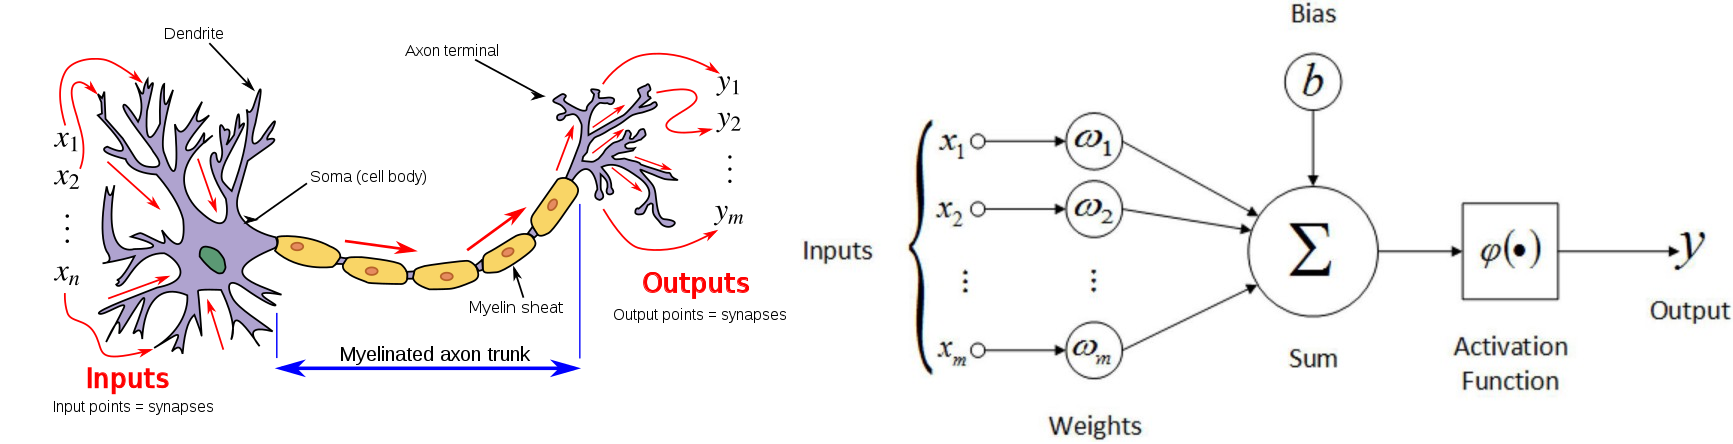
\includegraphics[width=\textwidth]{img/neuron_collage.png}
\end{figure}
From this, the simplest artificial network are just direct acyclic graphs, from an n-dimensional input to an m-dimensional output.
\begin{figure}[h]
    \caption{Image from \href{https://cs231n.github.io/convolutional-networks/}{CS231n}}
    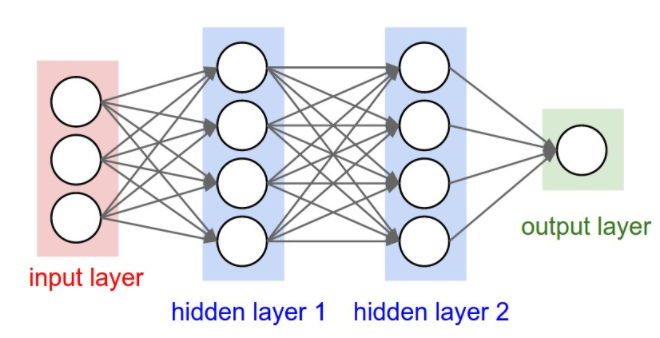
\includegraphics[width=\textwidth]{img/ANN.png}
\end{figure}
In an artificial network, the neuron usually computes a weighted sum of the inputs (the weights are what the network learns in training), `squishes' the result with a function (most often the sigmoid function, which constrains the output between 1 and 0), and shoots the result in the output. In equations, the result $y$ of the computation of a single neuron is calculated like this:
\begin{equation}
    y= \phi(\sum_{i=0}^{i=n}{x_i * \omega_i + b})
\end{equation}
Where $\phi$ is the `squishification' function (it can also be used to only consider the neuron active if its inputs are above a certain threshold!), $\omega_i$ are the weights, $x_i$ are the inputs and $b$ is the bias.

This already gives us enough information to understand simple multilayer perceptrons, and maybe even to imagine why the computational effort gets too great with hundreds of neurons interconnected. This is one of the two main reasons behind NN's `late bloom'; the other one is the available data.

\subsection{Underfitting and Overfitting}
Let us now consider two of the main issues all Neural Networks can have, and a couple ways to mitigate them: if a NN is not expressive enough, it will \textit{underfit} data. This means the function it learns to represent will be a far approximation of what it would take to recognize if a new input matches the training data, and is normally easily fixed by either increasing training time or deepening the network. The second, opposite issue common to NN is overfitting. Overfitting occurs when the network adapts too much to the training data, becoming too specific to it and refusing any input that does not match the training data exactly. This is a trickier problem to solve: simple solutions involve drop-off layers (layers in which sometimes some connections are ``severed'', so the network can't rely too much on any single neuron) or regularization (constraining the degree of freedom the network has).

\begin{figure}[h]
    \caption{Underfitting, fitting, and overfitting, from \href{https://www.geeksforgeeks.org/underfitting-and-overfitting-in-machine-learning/}{GeeksForGeeks} and \href{https://datascience.foundation/sciencewhitepaper/underfitting-and-overfitting-in-machine-learning}{DataScience Foundation}}
    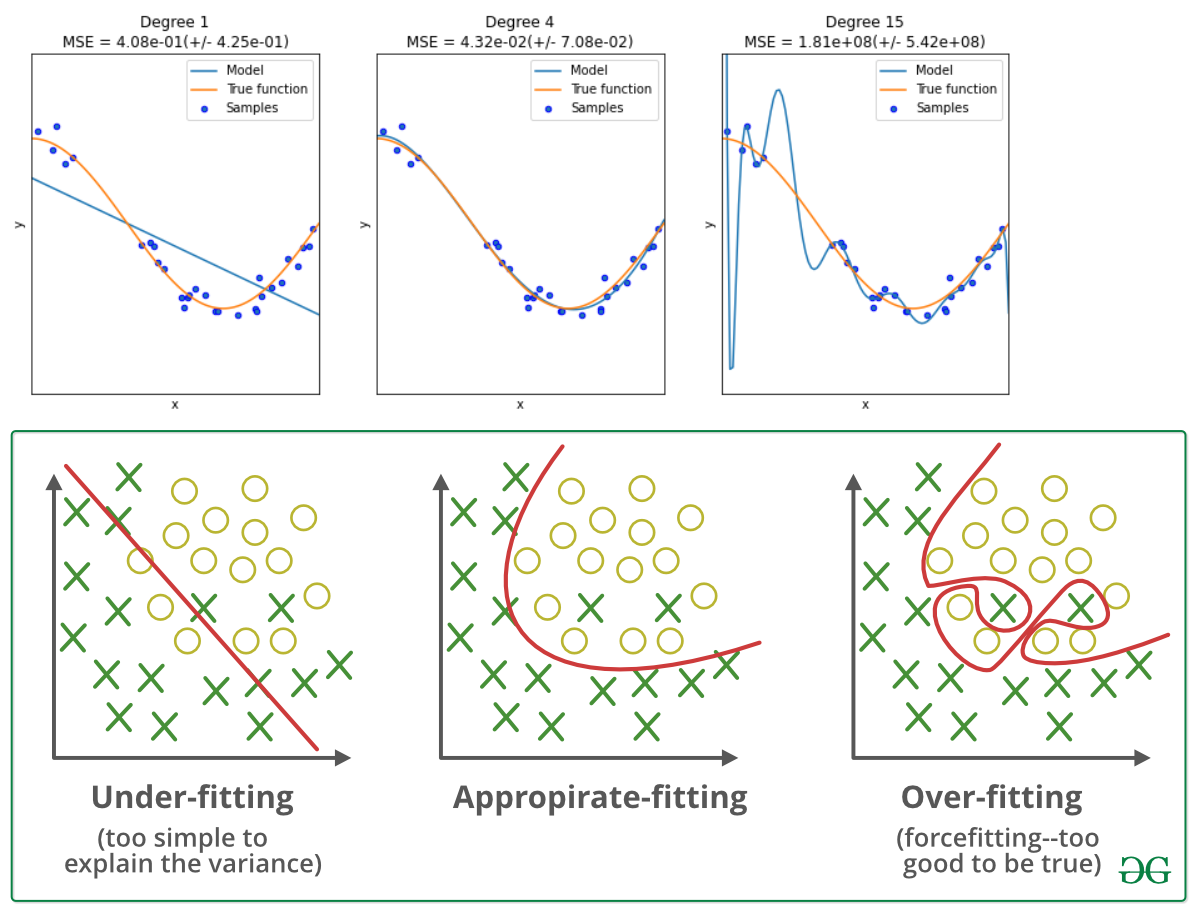
\includegraphics[width=\textwidth]{img/fitting_collage.png}
\end{figure}


\subsection{Additional concepts}
There are three more concepts relevant to us, that will help us understand network architectures: pooling, convolutions and recurrence.

\subsubsection{Pooling}
Pooling is a simple operation that reduces the dimension of the input: for every window of size $n\times n$, either the average value or the maximum value is taken. This has two effects: it regularizes the network, as it can't learn by using any specific input, and it reduces the number of free variables the network has to learn, as the final matrix is smaller than the input.

\subsubsection{Convolutions}
Assuming the reader is familiar with matrix multiplication, a convolution is a function that takes as input a kernel of size $n\times n$ and a matrix (in the case of NN, of neural activations), and only consists of computing the dot product between every `window' of size $n\times n$ with the kernel.
\begin{figure}[h]
    \caption{An example of convolving an image, from \href{https://en.wikipedia.org/wiki/Kernel_(image_processing)}{Wikipedia} }
    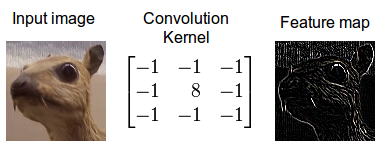
\includegraphics[width=\textwidth]{img/convolution.png}
\end{figure}

As it turns out, this simple operation is quite powerful: it allows to, for example on images, extract relevant features from an activation matrix, or sharpen or blur an image. When used in NN, kernels are not hard-coded to perform such tasks: they are learned by the network as it decides which features are relevant to solving its task. Convolutional layers are used in networks because of three important features:
\begin{enumerate}
    \item They take advantage of locality: because of their nature, they're able to easily express relationship between items that are close in the input, while perceptron treat all inputs as equidistant to each other.
    \item They reduce complexity: in multi-layer perceptrons, all inputs are connected to each other. In convolutional layer, they aren't. In addition, the filter is the same for the whole image: this drastically reduces the number of free parameters the network needs to learn.
    \item They can be used in conjuction with pooling layers: this grants them a degree of translational invariance, as the same result (or an average of the results) accounts for a region of the input, instead of a single point.
\end{enumerate}

As can be easily gleamed, convolutional networks are primarily used in visual recognition tasks: their characteristics and features are both apt to the task and were specifically developed for it; in fact, the original inspiration for them comes from the neuronal architecture of brain regions dedicated to visual processing.

\subsubsection{Recurrence}

Now, for recurrent networks. Recurrent networks were designed to tackle time-sequence problems, or tasks that require temporal context, often with long sequential data. As such, they process one element at a time (every time-step), and then pass the result of their computation to the next time step to facilitate the progress.
\begin{figure}[h]
    \caption{A recurrent unit, with its unrolled version. The three $s_{t-1}, s_t, s_{t+1}$ are the same unit in three different time steps \parencite{lecunDeepLearning2015}. }
    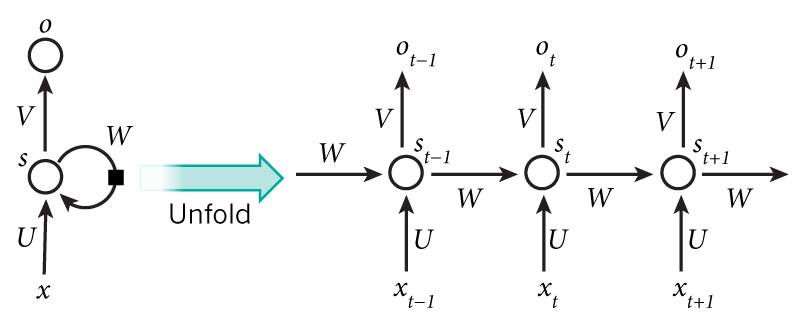
\includegraphics[width=\textwidth]{img/RNN.png}
\end{figure}
This type of recurrent neuron is only capable of limited time-context sizes: consider the phrase ``John went to pick up his truck and a bag of chips [...]. Later, \textit{he decided to...}''; as the size of [...] grows, the network's ability to predict the italics part dwindles to none, as it has to not only encode the information about the subject, but transmit it through multiple timesteps before using it. This is absolutely possible as hand-picked parameters, but networks have a hard time learning them.
\vspace{4pt}
\begin{wrapfigure}{r}{0.35\textwidth}
    \centering
    \caption{An LSTM cell, from \href{http://colah.github.io/posts/2015-08-Understanding-LSTMs/}{Christopher Olah's blog} }
    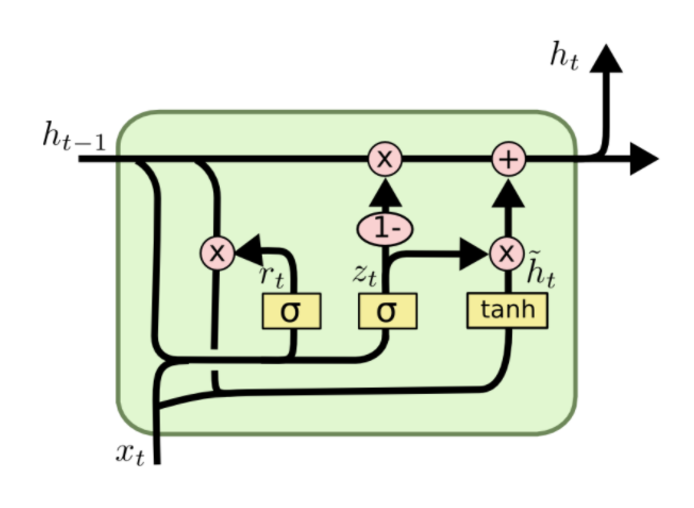
\includegraphics[width=0.35\textwidth]{img/LSTM.png}
\end{wrapfigure}

To tackle this, more complicated recurrent architectures were created. In the text, we mentioned LSTM (Long Short-Term Memory) cells. A much more complete introduction to them can be found \href{http://colah.github.io/posts/2015-08-Understanding-LSTMs/}{here}, a blog post so well-written it has become the unofficial standard introduction to LSTMs. What is relevant to us is that they do not have the long-term dependency issue we mentioned before, thanks to a gated \textit{cell state} and some simple forget and remember operation. Innumerent variations exist: as we mentioned in the text, this period of Deep Learning research does not stem from a focused and methodic mathematical search for optimized structures, but from successive approximations and intuitions.

\section{Additional Architectures and Features}
In this section, we will briefly go over some of the architectures in which networks are organized.

\textbf{Encoder-Decoder.} These models have one general characteristics: they are divided into two functional parts; the encoder forces the network to model the input into a (normally) lower-dimensional vector, which trains it to avoid noise; the decoder then translates this vector into a useful output. The specific characteristics of encoders and decoders don't really matter: with recurrent cell-based encoder and decoder, the network can approach variable-length tasks; with convolutional layers, the network becomes simple and quick to train (and can be further slimmed down by additional improvements like quantization); removing the decoder leaves the possible problem space mapped into a fixed-dimension vector, that can then be exported as a map in, for example, natural language processing tasks.

\textbf{Attention.} For a detailed explanation of some attention-based architectures, see \href{https://distill.pub/2016/augmented-rnns/}{distill.pub}. A simple explanation is that attention is a mechanism to let neural networks interact with other mediums, while keeping the interaction differentiable (hence learnable), whether the medium is a fixed memory (Neural Turing Machines), another RNN (Attentional Interfaces), or itself, by choosing how many times to `think' about a given input (Adaptive Computation Time). An example of an attention-based architecture is a Transformer.

\textbf{Generative Adversarial Networks.} GANs utilize two different networks: a generative network, which generates possible candidates, and a discriminative network, which evaluates them. This causes both of them to learn at the same time, and training is stopped when the discriminative gives the wrong answer about half the time. They were born as a way to train networks in unsupervised tasks, but they are now used in unsupervised, semi-supervised and supervised tasks.



\end{document}